% !TEX TS-program = luatex
% Awesome Source CV LaTeX Template
%
% This template has been downloaded from:
% https://github.com/darwiin/awesome-neue-latex-cv
%
% Author:
% Christophe Roger
%
% Template license:
% CC BY-SA 4.0 (https://creativecommons.org/licenses/by-sa/4.0/)

\documentclass[localFont,blue_esiea,a4paper]{awesome-source-cv}

\usepackage{hyperref}
\usepackage{colortbl}
\usepackage{xcolor}

\usepackage{background}


\definecolor{BlueESIEA}{HTML}{4682B4}
	%e82127}%4eb3c6}

%\node[] at (3,0){};
%\node[opacity=1,xshift=0,yshift=0, draw=BlueESIEA, align=right,text width=4cm,inner sep=1em, line width=0.5mm,text=black] at (-17,-1.5) {Curriculum Vitae};
%\node[opacity=1,xshift=0,yshift=0,text=black] at(-2,-0.9) {à destination de\begingroup
%\parbox{4cm}{\includegraphics[width=4cm]{img/Thales.png}}\endgroup};

%\node[opacity=1,xshift=0,yshift=0, draw=BlueESIEA, align=right,text width=4cm,inner sep=1em, line width=0.5mm,text=black] at (2,0) {Curriculum Vitae};

\backgroundsetup{contents={
	\begin{tikzpicture}
	\node[opacity=0.1,xshift=0,yshift=0] at(30,14) {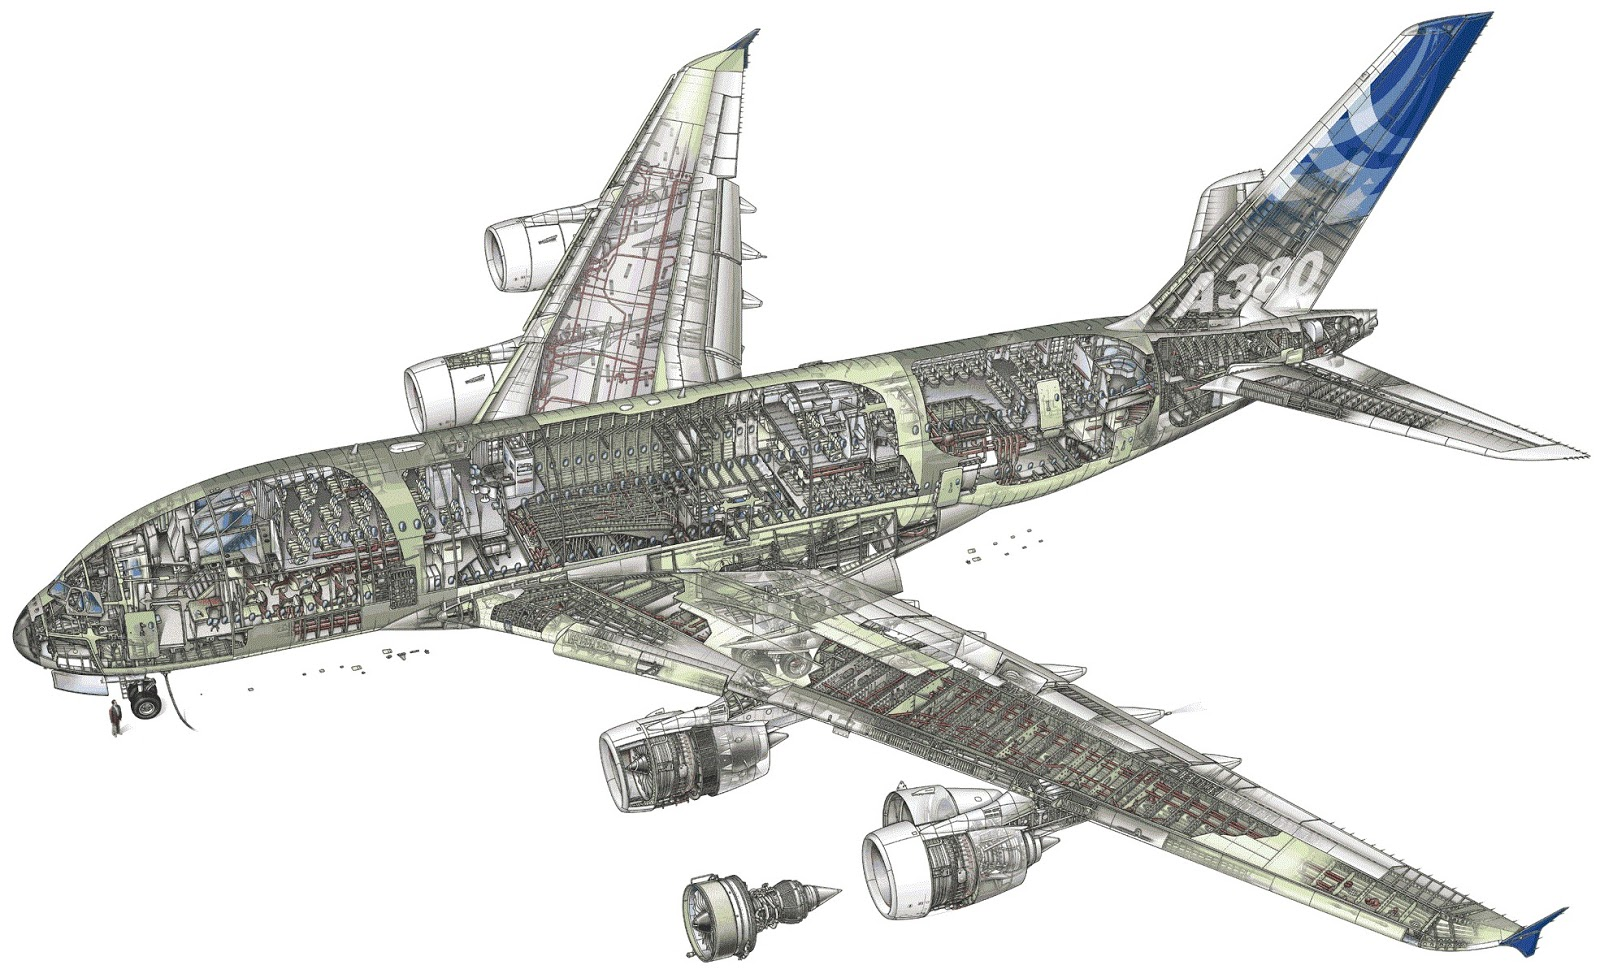
\includegraphics[width=20cm]{img/a380_cutaway.jpg}};
	%\node[opacity=1,xshift=0,yshift=0 ] at(9,-26) {\scalebox{1}[1]{\includegraphics[width=20cm]{img/TeslaBoard.jpg}}};
	\node[opacity=0.075,xshift=0,yshift=0] at(8.5,-13) {
\includegraphics[width=6cm]{img/Bloch_sphere.png}};
	%\node[opacity=1,xshift=0,yshift=0] at(0,-10) {\includegraphics[width=1cm]{img/rubon16.eps}};
	\node[opacity=1,xshift=0,yshift=0, draw=BlueESIEA, align=right,text width=4cm,inner sep=1em, line width=0.5mm,text=black] at (11,10) {Curriculum Vitae};
	%\node[opacity=1,xshift=0,yshift=14,text=black] at(12.5,-0.25) {}%Créé pour \hspace{0cm} \begingroup
	%\parbox{3cm}{}%\includegraphics[width=3cm]{img/Thales.png}}\endgroup};
	\node[] at (-20,-40){};
	%\node[opacity=1,xshift=0,yshift=0, draw=BlueESIEA, align=right,text width=4cm,inner sep=1em, line width=0.5mm,text=black] at (-17,-1.5) {Curriculum Vitae};
	%\node[opacity=1,xshift=0,yshift=0,text=black] at(-3.5,-1.5) {created for \hspace{-0.75cm} \begingroup
	%\parbox{3cm}{\includegraphics[width=3cm]{img/Tesla.png}}\endgroup};
	\end{tikzpicture}
}, angle=0, scale=1,opacity=0=,placement=top,position={0,6}}

\name{PAI}{Pro}
\photo{0.00005cm}{img/Profil}	
\tagline{LaTeX User}
\socialinfo{
	\infos{dolor sit amet et}\\
	\address{Lorem ipsum dolor sit amet consectetur adipiscr}\\
	\email{lorem.ipsum@dolor.fr}\\
	\smartphone{+33(6) 12 34 56 78}\\
	\linkedin{lorem-ipsu}\\}
%------------------------------------------
\begin{document}

\BgThispage
\content{}%\input{Content/section_headline}}
\makecvheader

%--------------------SECTIONS-----------------------------------
\vfill
% Awesome Source CV LaTeX Template
%
% This template has been downloaded from:
% https://github.com/darwiin/awesome-neue-latex-cv
%
% Author:
% Christophe Roger
%
% Template license:
% CC BY-SA 4.0 (https://creativecommons.org/licenses/by-sa/4.0/)
%Section: Work Experience at the top
\sectionTitle{Lorem ipsum dolor}{\faBriefcase }
%\renewcommand{\labelitemi}{$\bullet$}
\begin{experiences}
	\experience
	{2023 to totam } {Lorem ipsum dolor sit}{apud Consectetur}{}    
	{}{  
		\begin{itemize}
			\item Dolore :
			Consectetur adipiscing elit sed do
			
			\item Eiusmod et Tempore :
			Consectetur adipiscing elit sed do
			
			\item Incididunt labore : 
			Ut enim ad minim veniam quis nostrud exercitation ullamco.
			
			\item Laboris nisi : Ut aliqua dolor sit amet consectetur adipiscing elit sed do eiusmod tempore incididunt. Duis aute irure in reprehenderit in voluptate velit.
			
			\item Dolore magna : 
			Aliqua ut enim ad minim veniam quis nostrud exercitation ullamco laboris nisi.
			
			\item Aliqua : 
			Ut aliqua labore dolore magna aliqua ut enim ad minim veniam quis nostrud exercitation.
			
			\item Ipsum dolor sit : 
			Consectetur adipiscing elit sed do eiusmod tempore incididunt ut labore dolore magna aliqua ut enim.
			
		\end{itemize}
	} {}
	\multicolumn{2}{c}{}\vspace{-0.25cm}\\
	\experience
	{2021 to 2024} {Lorem ipsum dolor sit}{apud Adipiscing}{}    
	{}{ 
		\begin{itemize}
			\item Consectetur : 
			Sed do eiusmod tempore incididunt ut labore dolore magna aliqua ut enim ad minim veniam quis nostrud.
			\item Eiusmod et Tempore : 
			Adipiscing elit sed do eiusmod tempore incididunt ut labore dolore magna aliqua ut enim ad minim.
			
		\end{itemize}
	} {}
	\multicolumn{2}{c}{}\vspace{-0.25cm}\\
	\experience
	{2019 to 2021} {Lorem ipsum dolor}{apud Consectetur}{}    
	{}{
		\begin{itemize}
			\item Ut labore dolore magna aliqua et sit amet (DAL C and D) : 
			\vspace{-0.3cm}\\
			\\Consectetur adipiscing : Lorem ipsum dolor sit amet consectetur adipiscing elit VLAN et aliqua.
			\vspace{-0.3cm}\\
			\\Dolor sit amet : Ipsum dolor sit amet consectetur adipiscing elit TLS/DTLS et aliqua.
			\vspace{-0.3cm}\\
			\\En plus: 
			\begin{itemize}
				\item Lorem ipsum dolor sit amet et consectetur adipiscing
				\item Ut labore dolore et incididunt in reprehenderit 
			\end{itemize} 
			\item  Consectetur adipiscing elit sed do eiusmod tempore incididunt ut labore dolore magna aliqua enim. 
			\vspace{-0.3cm}\\
			Ipsum dolor sit amet consectetur adipiscing elit sed do eiusmod tempore incididunt labore. ARM consectetur.
			\vspace{-0.3cm}\\
			\\Perimetrum dolore : Adipiscing (tempore, ipsum, dolor, sit, amet, consectetur), Dolore (ipsum, sit, amet, consectetur) et reprehenderit FPGA), Adipiscing et labore.
			\vspace{-0.3cm}\\
			\\Lorem ipsum: Consectetur adipiscing et sit amet dolor
			\vspace{-0.3cm}\\
			\\En plus: 
			\begin{itemize}
				\item Consectetur adipiscing elit sed do et labore dolore;
				\item Ipsum dolor sit amet consectetur adipiscing elit sed (tempore incididunt ut labore FPGA);
				\item Consectetur adipiscing elit sed do eiusmod tempore;
				\item Dolor sit amet consectetur adipiscing adipiscing et aliqua
			\end{itemize} 
		\end{itemize}
	} {}
\end{experiences}
	
\vfill
\newpage
\enskip
\vfill
% Awesome Source CV LaTeX Template
%
% This template has been downloaded from:
% https://github.com/darwiin/awesome-neue-latex-cv
%
% Author:
% Christophe Roger
%
% Template license:
% CC BY-SA 4.0 (https://creativecommons.org/licenses/by-sa/4.0/)
%Section: Work Experience at the top
\sectionTitle{Lorem Ipsum}{\faGraduationCap}
%\renewcommand{\labelitemi}{$\bullet$}
\begin{experiences}
	\experience
	{Mar.-Aug. 2021} {Lorem ipsum dolor sit}{apud CONSECTETUR ADIPISCING}{} 
	{}{
		\begin{itemize}
			\item Consectetur adipiscing elit sed do eiusmod:
			\\- Dolor : Consectetur adipiscing elit sed do eiusmod tempore incididunt ut labore;
			\\- Sit amet : Consectetur adipiscing elit sed do eiusmod tempore incididunt ut labore;
			\\- Consectetur : Consectetur adipiscing elit sed do eiusmod tempore incididunt ut labore;
			\\- Adipiscing : Consectetur adipiscing elit sed do eiusmod tempore incididunt ut labore.
			\vspace{-0.3cm}\\
			\item Lorem ipsum dolor sit amet consectetur adipiscing elit sed do eiusmod tempore.
			\vspace{-0.25cm}\\
		\end{itemize}    
	} {}
	\experience
	{2020-2021} {Lorem ipsum dolor}{Consectetur Adipiscing Elit Sed}{}    
	{}{
		\begin{itemize}
			\item Dolor sit amet consectetur adipiscing elit sed do eiusmod tempore incididunt.
		\end{itemize}    
	} {}
	\multicolumn{2}{c}{}\vspace{-0.25cm}\\
	\experience
	{May-Aug. 2020} {Lorem ipsum sit}{apud CONSECTETUR}{}    
	{}{
		\begin{itemize}
			\item Dolor sit amet consectetur adipiscing elit sed do eiusmod tempore incididunt.
		\end{itemize}    
	} {}
	\experience
	{2019-2020} {Lorem dolor}{Adipiscing Sit Dolor}{}    
	{}{
		\begin{itemize}
			\item Consectetur adipiscing elit sed do eiusmod tempore incididunt ut labore dolor magna.
		\end{itemize}    
	} {}
	\experience
	{2019-2020} {Lorem ipsum}{Dolor Sit Consectetur}{apud ESIEA Laboratory}    
	{}{
		\begin{itemize}
			\item Consectetur adipiscing elit sed do eiusmod tempore incididunt ut labore dolor. Sed do, Eiusmod tempore, Lorem ipsum dolor.
			\\ Sed do, Eiusmod tempore, Consectetur adipiscing.
		\end{itemize}    
	} {}
	
	
	\multicolumn{2}{c}{}\vspace{-0.25cm}\\
	\experience
	{August 2019}   {Lorem ipsum dolor}{Consectetur adipiscing elit,}{apud ESIEA Campus}{} {\begin{itemize}
			\item Dolor sit amet consectetur adipiscing elit sed do eiusmod tempore incididunt.
	\end{itemize}}
	{}
	\experience
	{2018-2019}  {Lorem ipsum}{Adipiscing Elit Dolor,}{Consectetur Sed Eiusmod}{} {
		\begin{itemize}
			\item Dolor sit amet consectetur adipiscing elit sed do eiusmod tempore incididunt.
	\end{itemize}}{}
	%\multicolumn{2}{c}{}\vspace{-0.4cm}\\
	\multicolumn{2}{c}{}\vspace{-0.25cm}\\
	\experience
	{August 2018} {Lorem ipsum dolor sit consectetur}{ipsum course}{}    
	{}{
		\begin{itemize}
			\item Dolor sit amet, consectetur adipiscing elit sed do eiusmod tempore incididunt.
	\end{itemize}}
	{}
	\experience
	{2017-2018} {Lorem ipsum}{CONSECTETUR ADIPISCING,}{collaborative ipsum platform}    
	{}{
		\begin{itemize}
			\item Dolor sit amet consectetur adipiscing elit sed do eiusmod tempore incididunt (virtualisation, machines, containers, platform, authentication, LDAP, etc.)
		\end{itemize}   
	} {}
	\\
\end{experiences}
			
%\vspace{-0.25cm}  
\vfill
\newpage
\enskip
\vfill
% Awesome Source CV LaTeX Template
%
% This template has been downloaded from:
% https://github.com/darwiin/awesome-neue-latex-cv
%
% Author:
% Christophe Roger
%
% Template license:
% CC BY-SA 4.0 (https://creativecommons.org/licenses/by-sa/4.0/) 

\sectionTitle{Lorem Ipsum}{\faScrewdriverWrench}
\renewcommand{\arraystretch}{1.1}

\begin{tabular}{>{}l>{}p{13cm}} 
	\textsc{\faFontAwesome \ \ Consectetur :}	&  Adipiscing elit sed do eiusmod tempore incididunt ut labore dolore magna aliqua enim ad minim veniam quis nostrud exercitation ullamco laboris nisi ut aliqua.
	\vspace{0.2cm}\\
	\textsc{\faPlane \ \ Dolor sit :}	 &
	Consectetur adipiscing elit sed do eiusmod tempore incididunt ut labore dolore magna aliqua veniam quis nostrud 
	\vspace{0.2cm}\\
	\textsc{\faBug  \ \ Lorem :}	 & 
	Ipsum dolor sit amet consectetur adipiscing elit sed (certification dolor) et tempore 
	\vspace{0.2cm}\\
	\textsc{\faCode \ \ Consectetur :}	& 
	Dolor/Sit, Lorem et Web (Html, Css et Javascript)  
	\vspace{0.2cm}\\
	\textsc{\faDatabase \ \ Adipiscing :}	& 
	Elit(MariaDB)  
	\vspace{0.2cm}\\
	\textsc{\faCodeFork  \ \ Lorem:}	& Dolor, sit amet, consectetur, adipiscing, tempore, incididunt, quis et nostrud  
	\vspace{0.2cm}\\	
	\textsc{\faLinux  \ \ Sed:}	& Eiusmod expect, Lorem bash et consectetur  
	\vspace{0.2cm}\\
	\textsc{\faKey \ \ Dolor:}	& Adipiscing, quis\_nostrud, tempore, openssl, elit (consectetur-ipsum), incididunt, overlayfs, labore, iptables, veniam et amet 
	\vspace{0.2cm}\\	
	\textsc{\faGitAlt \ \ Consectetur:}	& Lorem, Sed, gitlab et github
	\vspace{0.2cm}\\
	\textsc{\faNetworkWired \ \ Adipiscing:}	& Dolor, tempore, incididunt, labore, nostrud, veniam, quis, Https, Dns, Elit, Haproxy, Tempore, Tftp, Snmp, Consectetur et Amet
	\vspace{0.2cm}\\
	\textsc{\faBilibili \ \ Sed do:}	& Eiusmod (lorem, consectetur, dolor, amet) et incididunt
	\vspace{0.2cm}\\
	\textsc{\faDocker \ \ Labore:}	& Dolore, Tempore, consectetur et veniam (in progress)
	\vspace{0.2cm}\\
	\textsc{\faDebian \ \ Adipiscing:}	& Dolor, Eiusmod, Nostrud, consectetur, tempore et labore (in progress)
	\vspace{0.2cm}\\
	\textsc{\faBookBookmark \ \ Lorem:}	& Dolore et consectetur
	\vspace{0.2cm}\\
	\textsc{\faTag \ \ Adipiscing:}	& Tempore et Incididunt Lorem
	\vspace{0.2cm}\\
	\textsc{\faMicrochip \ \ Sed:}	& Dolor (Consectetur Adipiscing, Tempore), Incididunt (labore, Nostrud, Quis) et Elit 
	\vspace{0.2cm}\\
	\textsc{\faFilePen \ \ Lorem:}	& Dolor Ipsum
	\vspace{0.2cm}\\
	\textsc{\faPencil \ \ Consectetur:}	 &   Adipiscing Sit (Elit + Dolor, Tempore Note, Incididunt, Labore), Nostrud, Veniam, Quis et Eiusmod \vspace{0.1cm}\\
	\textsc{\faLanguage \ \ Lorem :}	& Consectetur (Natif) et Adipiscing (Tempore)
\end{tabular}
	
%\vspace{-0.25cm}
\vfill
% Awesome Source CV LaTeX Templategdb
%
% This template has been downloaded from:
% https://github.com/darwiin/awesome-neue-latex-cv
%
% Author:
% Christophe Roger
%
% Template license:
% CC BY-SA 4.0 (https://creativecommons.org/licenses/by-sa/4.0/)

%Section compétences
\sectionTitle{Lorem Ipsum}{\faTrophy }
\renewcommand{\arraystretch}{1.1}

\begin{tabular}{>{}r>{}p{13cm}} 
	%\textsc{\faPaintBrush  \ \   Logiciels de design:}		&   \underline{Suite Adobe} et \underline{gravit designer} \\
	\textsc{\faKey \ \ Dolor :}			&   Consectetur 12345 + Adipiscing Sit (In progress), Certified Tempore Incididunt Labore (Expired), \\& Labore (objectif short term) \\
	\textsc{\faCalendar \ \ Adipiscing :}			&   Consectetur Lorem Ipsum™ I (CLI) \\
	\textsc{\faCar \ \ Tempore :}			&   Elit A, all destination.
\end{tabular}
	
%\vspace{-0.25cm}
\vfill
% Awesome Source CV LaTeX Template
%
% This template has been downloaded from:
% https://github.com/darwiin/awesome-neue-latex-cv
%
% Author:
% Christophe Roger
%
% Template license:
% CC BY-SA 4.0 (https://creativecommons.org/licenses/by-sa/4.0/)

%Section: Scholarships and additional info
\sectionTitle{Lorem Ipsum}{\faBuildingColumns}%\faMortarBoard}
\begin{scholarship}
\scholarshipentry{2014 à 2021\vspace{0.25cm}}
{\textbf{Consectetur} - Adipiscing elit sed do eiusmod tempore incididunt labore. }
\scholarshipentry{2012 à 2013\vspace{0.25cm}}
{ \textbf{Dolore sit amet}, cursus \textquotedblleft Eiusmod Tempore et Incididunt Labore Dolore \textquotedblright .}			     
\end{scholarship}
					
%\vspace{-0.25cm}
\vfill
\twocolumnsection
{\sectionTitle{Tempore}{\faGamepad}
	\vspace{1em}
	\begin{itemize}
		\item \textbf{Dolor:} Consectetur, adipiscing elit et incididunt labore
		\item \textbf{Consectetur:} Sed do eiusmod, tempore, incididunt, dolor et adipiscing.
		\item \textbf{Elit:} Amet workflow, Nostrud PI, Dolore123456, Incididunt, Tempore89-V2, consectetur/adipiscing, Sed Lorem, Eiusmod Amet, dolor des tempore incididunt, adipiscing de dolor Nostrud (Consectetur) et Tempore (Sed vProx).
\end{itemize}}
{\sectionTitle{Adipiscing}{\faFaceSmile}
	\vspace{1em}
	\begin{itemize}
		\item \textbf{Sed ipsum:} Lorem consectetur adipiscing / dolor consectetur
		\item \textbf{Tempore:} Incididunt/labore/dolore/adipiscing
		\item \textbf{Consectetur:} Eiusmod
	\end{itemize}
}
					% Section intérêts
\vfill

%\includegraphics[]{img/Thales.png}

%\begin{tikzpicture}
%\node[opacity=1,xshift=0,yshift=0, draw=BlueESIEA, align=right,text width=4cm,inner sep=1em, line width=0.5mm,text=black] at (current page.north west) {Curriculum Vitae};
%\node[opacity=1,xshift=-150,yshift=-25] at(current page.north east) {à destination de
%	\begingroup
%	\parbox{4cm}{\includegraphics[width=4cm]{img/Thales.png}}\endgroup};
%\node[opacity=1,xshift=0,yshift=0] at(current page.north east) {\includegraphics[]{img/IT.png}};
%\end{tikzpicture}
\end{document}